% ============================================================
% Lecture 14 -- Fundamentals of matrices
% ============================================================
\section{Fundamentals of Matrices and the Projection $P_X$}\label{sec:L14}

\lectureheader{14}{K_j3NHsQ4t8}{Week-4 handwritten notes \texttt{Feb14.pdf}, part ``Lecture 4'' (proposition on $X\beta$ and $P_X$; linear algebra review of the four subspaces, $\nullsp{A}=\nullsp{A\T A}$, rank--nullity)}

\begin{guiding*}
By the end of this lecture you should be able to:
\begin{itemize}
  \item show that $X\beta$ is estimable and that its least squares estimate is $X\hat\beta=\PX Y$, the orthogonal projection of $Y$ onto $\colsp{X}$;
  \item work with the four fundamental subspaces of a matrix, and compute them for small examples;
  \item prove $\nullsp{A}=\nullsp{A\T A}$ and $\colsp{A\T A}=\colsp{A\T}$ using the rank--nullity theorem;
  \item construct $\PX$ and list its properties.
\end{itemize}
\end{guiding*}

\subsection{Recap}
Least squares estimates are the solutions of $X\T X\beta=X\T Y$ (\cref{thm:L12-normal}). The estimate of $\lambda\T\beta$
is unique exactly when $\lambda\T\beta$ is estimable (\cref{thm:L13-unique}). Both proofs used
$\colsp{X\T X}=\colsp{X\T}$ (\cref{lem:L12-colspace}). This lecture proves it and identifies the fitted vector
geometrically.

\subsection{$X\beta$ and the orthogonal projection}
\begin{definition}[Orthogonal projection]\label{def:L14-proj}
Let $V\subseteq\RR^n$ be a subspace. A vector $w\in V$ is the \vocab{orthogonal projection} of $y\in\RR^n$ onto $V$ if
$y-w\perp V$, i.e.\ $\langle y-w,v\rangle=0$ for all $v\in V$. The matrix $P_V$ with $P_Vy=$ (projection of $y$) is the
\vocab{orthogonal projection matrix} onto $V$. For $V=\colsp{X}$ we write $\PX$.
\end{definition}

\begin{lemma}[Projection theorem]\label{lem:L14-projection}
For every subspace $V$ and every $y\in\RR^n$ the orthogonal projection $w$ exists and is unique. It is the unique
closest point of $V$ to $y$: $\pnorm{y-v}^2=\pnorm{y-w}^2+\pnorm{w-v}^2$ for all $v\in V$. The map $y\mapsto w$ is linear,
given by the matrix $P_V=\sum_{i=1}^r u_iu_i\T$ for any orthonormal basis $u_1,\dots,u_r$ of $V$. The matrix is symmetric and
idempotent ($P_V\T=P_V=P_V^2$), with $\colsp{P_V}=V$ and $\rank P_V=\tr P_V=\dim V$.
\end{lemma}
\begin{proof}
Choose an orthonormal basis $u_1,\dots,u_r$ of $V$ (Gram--Schmidt) and put $w=\sum_i(u_i\T y)u_i\in V$. For each $j$,
$u_j\T(y-w)=u_j\T y-\sum_i(u_i\T y)u_j\T u_i=u_j\T y-u_j\T y=0$. So $y-w$ is orthogonal to every basis vector, hence to $V$.
\emph{Uniqueness:} if $w,w'\in V$ both have $y-w,\ y-w'\perp V$, then $w-w'=(y-w')-(y-w)\in V\cap V^\perp$. So
$\pnorm{w-w'}^2=\langle w-w',w-w'\rangle=0$.
\emph{Closest point:} for $v\in V$, $y-v=(y-w)+(w-v)$ with $w-v\in V\perp y-w$, and expanding the square gives the
identity. \emph{Matrix:} $w=\sum_iu_i(u_i\T y)=\bigl(\sum_iu_iu_i\T\bigr)y$, so $P_V=\sum_iu_iu_i\T$. It is clearly symmetric, and
$P_V^2=\sum_{i,j}u_i(u_i\T u_j)u_j\T=\sum_iu_iu_i\T=P_V$. Its columns lie in $V$, and $P_Vu_j=u_j$, so $\colsp{P_V}=V$. Finally,
$\tr P_V=\sum_i\tr(u_iu_i\T)=\sum_iu_i\T u_i=r$.
\end{proof}

\begin{proposition}\label{prop:L14-PX}
In the linear model $(Y,X\beta,\sigma^2I_n)$, $X\beta$ is estimable (every component is), and its least squares estimate is
\[
X\hat\beta=\PX Y .
\]
\end{proposition}
\begin{proof}
$X\beta=(x_1\T\beta,\dots,x_n\T\beta)\T$, where $x_i\T$ is the $i$th row of $X$. Since $x_i=X\T e_i\in\colsp{X\T}$, every component is
estimable (\cref{thm:L10-estimable}). (The notes leave this as an exercise; $\EE[Y_i]=x_i\T\beta$ shows it directly.)
Let $\hat\beta$ solve the normal equations. By \cref{thm:L12-normal},
\[
R_0^2=\pnorm{Y-X\hat\beta}^2=\min_{\beta\in\RR^p}\pnorm{Y-X\beta}^2=\min_{v\in\colsp{X}}\pnorm{Y-v}^2 .
\]
Since $X\hat\beta\in\colsp{X}$, it is a closest point of $\colsp{X}$ to $Y$. By \cref{lem:L14-projection} the closest point is unique
and equals $\PX Y$. Hence $X\hat\beta=\PX Y$ and $R_0^2=\pnorm{Y-\PX Y}^2$.
(Alternatively: $X\hat\beta\in\colsp{X}$, and $Y-X\hat\beta\perp\colsp{X}$ because $X\T(Y-X\hat\beta)=0$; this is the definition of the projection.)
\end{proof}

\subsection{Linear algebra review: the four fundamental subspaces}
For an $m\times n$ matrix $A$ (a map $\RR^n\to\RR^m$, $x\mapsto Ax$):
\begin{itemize}
  \item \vocab{column space} $\colsp{A}=\{Ax:x\in\RR^n\}=\{b\in\RR^m:Ax=b\text{ has a solution}\}\subseteq\RR^m$;
  \item \vocab{null space} $\nullsp{A}=\{x\in\RR^n:Ax=0\}\subseteq\RR^n$;
  \item \vocab{row space} $\rowsp{A}=\colsp{A\T}\subseteq\RR^n$;
  \item \vocab{left null space} $\nullsp{A\T}\subseteq\RR^m$.
\end{itemize}
The \vocab{rank} of $A$ is $\dim\colsp{A}=\dim\rowsp{A}$ (the number of linearly independent columns, equal to the number of independent
rows). The \vocab{nullity} is $\dim\nullsp{A}$. The row space and the null space are orthogonal complements in $\RR^n$, and $\colsp{A}$ and
$\nullsp{A\T}$ are orthogonal complements in $\RR^m$.

\begin{theorem}[Rank--nullity]\label{thm:L14-ranknullity}
For an $m\times n$ matrix $A$, $\rank(A)+\dim\nullsp{A}=n$.
\end{theorem}
\begin{proof}
Let $v_1,\dots,v_s$ be a basis of $\nullsp{A}$ and extend it to a basis $v_1,\dots,v_n$ of $\RR^n$. Every $Ax$ is a combination of
$Av_{s+1},\dots,Av_n$, because $Av_1=\dots=Av_s=0$. These vectors are independent: if $A\sum_{i>s}c_iv_i=0$, then
$\sum_{i>s}c_iv_i\in\nullsp{A}=\mathrm{span}\{v_1,\dots,v_s\}$, which forces all $c_i=0$ by the independence of $v_1,\dots,v_n$. So
$\rank A=n-s$.
\end{proof}

\begin{example}[The four subspaces of a rank-one matrix]\label{ex:L14-subspaces}
The example on the board is only partly legible in the published notes. It is a $2\times 3$ matrix whose
column space is $\{b:b_2=2b_1\}$. We take
\[
A=\begin{pmatrix}1&2&1\\2&4&2\end{pmatrix}.
\]
\begin{itemize}
  \item $\colsp{A}$: every column is a multiple of $(1,2)\T$, so $\colsp{A}=\mathrm{span}\{(1,2)\T\}$. By row reduction, $Ax=b$ is solvable iff
  $R_2-2R_1$ gives $0=b_2-2b_1$, i.e.\ iff $b_2=2b_1$ (e.g.\ $b=(1,2)\T$). The rank is $1$.
  \item $\rowsp{A}=\colsp{A\T}=\mathrm{span}\{(1,2,1)\T\}$, a line in $\RR^3$.
  \item $\nullsp{A}=\{x:x_1+2x_2+x_3=0\}=\mathrm{span}\{(-2,1,0)\T,(-1,0,1)\T\}$, a plane in $\RR^3$ orthogonal to $(1,2,1)\T$.
  \item $\nullsp{A\T}=\{y:y_1+2y_2=0\}=\mathrm{span}\{(2,-1)\T\}$, orthogonal to $\colsp{A}$ in $\RR^2$.
  \item Rank--nullity: $1+2=3=n$.
\end{itemize}
\end{example}

\begin{figure}[ht]
\centering
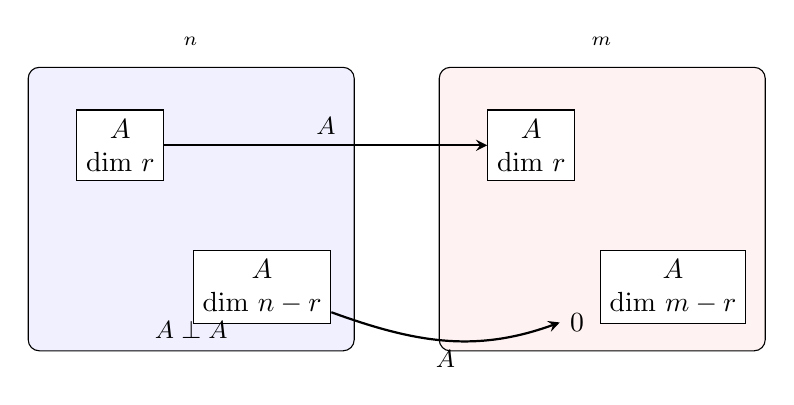
\begin{tikzpicture}[scale=0.9,>=stealth]
\draw[rounded corners,fill=blue!6] (-5.2,-1.8) rectangle (-0.6,2.2);
\node at (-2.9,2.5) {$\RR^n$};
\node[draw,fill=white,align=center] (R) at (-3.9,1.1) {$\rowsp{A}$\\dim $r$};
\node[draw,fill=white,align=center] (N) at (-1.9,-0.9) {$\nullsp{A}$\\dim $n-r$};
\draw[rounded corners,fill=red!5] (0.6,-1.8) rectangle (5.2,2.2);
\node at (2.9,2.5) {$\RR^m$};
\node[draw,fill=white,align=center] (C) at (1.9,1.1) {$\colsp{A}$\\dim $r$};
\node[draw,fill=white,align=center] (NT) at (3.9,-0.9) {$\nullsp{A\T}$\\dim $m-r$};
\draw[->,thick] (R) -- node[above,font=\small] {$A$} (C);
\draw[->,thick] (N) to[out=-20,in=-160] node[below,font=\small] {$A$} (2.3,-1.4) node[right] {$0$};
\node[font=\small] at (-2.9,-1.5) {$\rowsp{A}\perp\nullsp{A}$};
\node[font=\small] at (2.9,-1.5) {};
\end{tikzpicture}
\caption{The four fundamental subspaces. $A$ maps the row space one-to-one onto the column space and kills the null space.}
\label{fig:L14-four}
\end{figure}

\begin{theorem}\label{thm:L14-colspace}
For every $m\times n$ matrix $A$:
\begin{enumerate}
  \item $\nullsp{A}=\nullsp{A\T A}$;
  \item $\rank(A\T A)=\rank(A)$;
  \item $\colsp{A\T A}=\colsp{A\T}$.
\end{enumerate}
In particular, \cref{lem:L12-colspace} holds.
\end{theorem}
\begin{proof}
(1) If $x\in\nullsp{A}$, then $Ax=0$, so $A\T Ax=0$ and $x\in\nullsp{A\T A}$. Conversely, if $A\T Ax=0$, then
\[
0=x\T A\T Ax=\langle Ax,Ax\rangle=\pnorm{Ax}^2 ,
\]
so $Ax=0$ and $x\in\nullsp{A}$.
(2) $A$ and $A\T A$ both have $n$ columns. By rank--nullity and (1),
$\rank(A\T A)=n-\dim\nullsp{A\T A}=n-\dim\nullsp{A}=\rank(A)$.
(3) $\colsp{A\T A}\subseteq\colsp{A\T}$, because $A\T Ax=A\T(Ax)$. Both spaces have dimension $\rank(A\T A)=\rank(A)=\rank(A\T)$
by (2). A subspace contained in another of the same finite dimension equals it.
\end{proof}
\begin{note}
The notes add: ``in the recording it was mentioned $\colsp{A}$ instead of $\colsp{A\T}$''. The correct statement
is $\colsp{A\T A}=\colsp{A\T}$, a subspace of $\RR^n$. The spaces $\colsp{A\T A}$ and $\colsp{A}$ in general lie in
different spaces ($\RR^n$ versus $\RR^m$). Note also that $\colsp{AA\T}=\colsp{A}$, by the theorem applied to $A\T$.
\end{note}

\subsection{A formula for $\PX$}
\begin{proposition}[Supplementary: $\PX$ via a generalized inverse]\label{prop:L14-PXformula}
For any generalized inverse $\ginv{(X\T X)}$,
\[
\PX=X\ginv{(X\T X)}X\T ,
\]
and this matrix does not depend on the choice of generalized inverse. If $\rank X=p$, then $\PX=X(X\T X)^{-1}X\T$.
\end{proposition}
\begin{proof}
Let $G=\ginv{(X\T X)}$. By the note in \cref{sec:L12}, $\hat\beta=GX\T Y$ solves the normal equations for every $Y$. By
\cref{prop:L14-PX}, $XGX\T Y=X\hat\beta=\PX Y$ for all $Y$, so $XGX\T=\PX$. The right-hand side is the unique projection matrix, so it
does not depend on $G$.
\end{proof}

\begin{example}[$\PX$ in the one-way model]\label{ex:L14-PXoneway}
For \cref{ex:L12-oneway} ($k=2$, $n_1=n_2=2$), $\colsp{X}$ is spanned by the orthonormal vectors
$u_1=\frac1{\sqrt2}(1,1,0,0)\T$ and $u_2=\frac1{\sqrt2}(0,0,1,1)\T$. So
\[
\PX=u_1u_1\T+u_2u_2\T=\begin{pmatrix}\tfrac12&\tfrac12&0&0\\\tfrac12&\tfrac12&0&0\\0&0&\tfrac12&\tfrac12\\0&0&\tfrac12&\tfrac12\end{pmatrix},
\qquad \PX Y=\PX\begin{pmatrix}3\\5\\8\\10\end{pmatrix}=\begin{pmatrix}4\\4\\9\\9\end{pmatrix}=X\hat\beta(t)\ \ \forall t .
\]
$\tr\PX=2=\rank X$. The residual is $(I-\PX)Y=(-1,1,-1,1)\T$ and $R_0^2=4$. With $G=\mathrm{diag}(0,\tfrac12,\tfrac12)$
(\cref{prob:L12-4}), $XGX\T$ gives the same matrix.
\end{example}

\subsection{Computation}
\nb{week04/L14\_matrices\_projection.ipynb} computes the four subspaces of \cref{ex:L14-subspaces} with
\texttt{scipy.linalg.null\_space} and \texttt{orth}. It verifies $\nullsp{A}=\nullsp{A\T A}$ and the rank identities on random
rank-deficient matrices, builds $\PX$ in three ways (orthonormal basis, $X(X\T X)^{+}X\T$, $X\,\ginv{(X\T X)}X\T$ with a
hand-made $G$), and checks symmetry, idempotence and trace.

\subsection{Summary}
\begin{itemize}
  \item $X\beta$ is estimable, and its least squares estimate is $X\hat\beta=\PX Y$, the orthogonal projection of $Y$ onto $\colsp{X}$.
  \item $\PX=\sum u_iu_i\T=X\ginv{(X\T X)}X\T$: symmetric, idempotent, trace $=\rank X$.
  \item $\nullsp{A}=\nullsp{A\T A}$, $\rank A\T A=\rank A$, $\colsp{A\T A}=\colsp{A\T}$ (rank--nullity).
  \item $\rowsp{A}\perp\nullsp{A}$ in $\RR^n$ and $\colsp{A}\perp\nullsp{A\T}$ in $\RR^m$.
\end{itemize}

\subsection{Exercises}
\begin{problem}\label{prob:L14-1}
Show that $I-\PX$ is the orthogonal projection onto $\colsp{X}^\perp=\nullsp{X\T}$, and that $\PX(I-\PX)=0$.
\end{problem}
\begin{problem}\label{prob:L14-2}
Compute $\PX$ for simple linear regression with $x=(1,2,3,4)$ and verify that $\PX Y=(1.9,3.3,4.7,6.1)\T$ for $Y=(2,3,5,6)\T$.
\end{problem}
\begin{problem}\label{prob:L14-3}
For the one-way model with general $k$ and $n_i$, show that $\PX$ is block diagonal with blocks $\frac1{n_i}\one_{n_i}\one_{n_i}\T$, and that $(\PX Y)_{ij}=\bar Y_{i\cdot}$.
\end{problem}
\begin{problem}\label{prob:L14-4}
Find the four fundamental subspaces of $B=\begin{pmatrix}1&0&1\\0&1&1\end{pmatrix}$ and check rank--nullity.
\end{problem}
\begin{problem}\label{prob:L14-5}
Prove that if $P$ is symmetric and idempotent, then $P$ is the orthogonal projection onto $\colsp{P}$.
\end{problem}

\subsection{Further reading}
Christensen, Appendix~A (vector spaces), Appendix~B.3 (projections) and \S2.2; Rao, \S1a--1c (vector spaces,
matrices, projection operators) and \S4a.
